\pagestyle{empty}
	\cleardoublepage
\pagestyle{fancy}


\chapter{Estator Externo e Rotor}

A parte passiva do mancal magnético, composta pelo estator externo e pelo rotor,  pode ser descrita como o circuito da Fig. \ref{Fig:Modelagem:circuito:passivo:umlado}, onde um ímã permanente gera um fluxo magnético ($\mathcal{F}_c$) que estabiliza o eixo axial (passivo). O caminho principal desse fluxo é através do entreferro ($R_{ge}$) tanto pelos ferros do estator ($R_{ef}$) quanto pelos ferros do rotor ($R_{rf}$ e $R_{rr}$). Dois caminhos extras são considerados, um de vazamento de fluxo magnético no ímã ($R_{lm}$) e outro em cada entreferro ($R_{lg}$). 

\begin{figure}[!ht]
	\centering
	\def\svgwidth{1\columnwidth}
	\includesvg{modelo_circuito_passivo_umlado}
	\caption{Circuito magnético passivo suposto}
	\label{Fig:Modelagem:circuito:passivo:umlado}
\end{figure}

Um modelo fenomenológico foi inicialmente criado e nele aplicado um algorítimo de otimização a fim de encontrar um mancal ótimo para um certo funcional que valoriza as especificações anteriores. Com as dimensões encontradas, um modelo em elementos finitos foi gerado e as constantes de força calculadas de maneira mais precisa.

\section{Modelagem Magnética}

Nesse modelo, o ímã é considerado como uma fonte de fluxo magnético na forma equivalente a um circuito Thevenin. A força magnética coerciva ($\mathcal{F}_c$) representa a força magnética necessária para levar o ímã permanente a produzir um fluxo magnético nulo. Ímãs de terra rara (Samário Cobalto - Neodímio), possuem tipicamente uma curva linear de magnetização no segundo quadrante, essa curva depende de duas constantes físicas que variam com o material usado: $H_c$ constante que associa o comprimento do ímã com a força coerciva ($ F_c = H_c \, l_m$) e $B_r$ que descreve o fluxo máximo do ímã num cenário de curto circuíto ($\phi_r = B_r \, A_m$), ilustrada na Fig. \ref{Fig:Modelagem:circuito:passivo:ima}.

\begin{figure}[!ht]
	\centering
	\def\svgwidth{0.7\columnwidth}
	\includesvg{modelo_circuito_passivo_ima}
	\caption{Curva de desmagnetização típica de ímãs de terra rara}
	\label{Fig:Modelagem:circuito:passivo:ima}
\end{figure}

A curva de magnetização é descrita como :

\begin{align}
B_m = B_r + \frac{B_r}{H_c} H_m
\label{eq:p:ima}
\end{align}

A relação $\frac{B_r}{H_c}$ pode ser interpretada como a permeabilidade do meio (ímã) e possui tipicamente um valor próximo da permeabilidade do vácuo, $\mu_0$. O ponto de operação do ímã depende da curva de carga do circuíto magnético em que ele está inserido, para isso é necessário primeiramente calcular o valor da permeabilidade total e então identificar o ponto de operação do ímã e o seu fluxo produzido.

Considera-se nesse modelo para os materiais ferros magnéticos a curva de magnetização do ferro 1020, a curva não linear é apresentada na Fig. \ref{Fig:Modelagem:BH}, nota-se que a saturação ocorre por volta de 1.3T. Essa relação pode ser descrita como:

\begin{align}
B(H) = \mu(H) \, H
\label{eq:p:BH:ferro}
\end{align}

\begin{figure}[!ht]
	\centering
	\caption*{ Vetor campo magnético (T) x Campo Magnético (A/m)}
	\includegraphics[width=0.6\linewidth]{modelo_curva_bh}
	\caption{Curva de magnetização para o ferro 1020}
	\label{Fig:Modelagem:BH}
\end{figure}


\subsection{Campo Magnético no Entreferro}

A relutância magnética é proporcional ao comprimento da linha de campo no meio e inversamente proporcional a permeabilidade do meio e a área em que o campo está disperso. Com isso, calcula-se as relutância principais do circuíto :

\begin{align}
R_{p}  &= \frac{h_m}{\mu_m \, S_m}			\\
R_{ef} &= \frac{w_{ef}}{\mu_{ef}\, S_{ef}}  \\     
R_{rf} &= \frac{w_{rf}}{\mu_{rf}\, S_{rf}}   \\    
R_{rr} &= \frac{h_m}{\mu_{rr} \, S_{rr}}     \\      
R_{ge} &= \frac{l_g}{\mu_0  \, S_{ge}}        
\end{align}

A permeância gerada pelo vazamento pode ser calculada por \citep{Leupold1996a}: 

\begin{align}
P_{lm} &= \frac{0.64 \,  \mu_0 \,r_{ee}}{h_m/(h_m+2h_{ef})+1} \\
R_{lg} &= P_1 + P_2 + P_3 + P_4	
\end{align} 

Sendo $R_{g//}$ a associação paralela entre a relutância do entreferro e o vazamento associado, $R_1$ a soma das relutâncias do circuíto principal e $R_T$ a associação entre todas as relutâncias do circuíto. $\phi_1$ é o fluxo magnético na primeira malha e $\phi_2$ o fluxo magnético na malha principal. Obtém-se as seguintes equações:

\begin{align}
\phi_m &= \phi_1 + \phi_2 \\
&= \frac{F_c}{R_p + R_T} \\
\mathcal{F}_c	 &= \phi_1 \, (R_p + R_1) \\
\mathcal{F}_c    &= \phi_2 \, (R_p + R_{lm})
\end{align}

Encontra-se o campo magnético efetivo no entreferro:

\begin{align}
\phi_{ge} &= \frac{\phi_1 \, R_{lg}}{R_{ge}+R_{lg}} \\
B_{ge} &= \frac{\phi_g}{S_{ge}}
\end{align}


\subsection{Decomposição do Vetor Campo Magnético B em X e Z} \label{SubSec:CampoX/Y}

O campo magnético acumulado no entreferro pode ser decomposto em componentes $B_x$ e $B_z$ que dependem do deslocamento do rotor em $\Delta_x$ e $\Delta_z$. Esse deslocamento implica também em um aumento no comprimento do entreferro: $l_g$. A Fig. \ref{Fig:modelo:passivo:DxDz} ilustra o deslocamento. Tal modelo não leva en consideração o \textit{tilt} do rotor, o que implicaria em relutâncias diferentes para a parte superior e inferior do entreferro, já que os comprimentos seriam diferentes. 

\begin{figure}[!ht]
	\centering
	\def\svgwidth{0.6\columnwidth}
	\includesvg{modelo_passivo_DxDy}
	\caption{Deslocamento em X e Y}
	\label{Fig:modelo:passivo:DxDz}
\end{figure}

Os campos podem então ser derivados:

\begin{align}
\theta_z &= tg^{-1}(\frac{\Delta_z}{\Delta_x}) \\
l_g &= \sqrt{\Delta_x^2 + \Delta_z^2} \\
B_{gx} &= B \, cos(\theta_z) \\
B_{gz} &= B \, sin(\theta_z) 
\end{align}


\section{Força}

A força magnética de atração do rotor pelo estator é gerada pela energia eletromagnética acumulada no entreferro (superior e inferior), essa força pode ser calculada através do trabalho virtual \citep{Chiba}:

\begin{align}
|\vec{F}(l_g)| &=  \frac{ \vec{B}_{g}^2 \; S_g}{2 \, \mu_0} \label{eq:passivo:Fx}
\end{align}

A força resultante de atração é composta pela força dos dois entreferros (superior e inferior) que possuem mesmo módulo e intensidade já que os deslocamentos são simétricos. 

\subsection{Força Radial} \label{subsection:forca:x}


Visando obter as resultantes das forças projetadas nos eixos radiais (x e y), para alcançarmos um modelo mais preciso das forças, o mancal foi dividido em oito partes distintas sendo que cada parte possuía um componente de campo magnético diferente das outras partes. Para que obtivéssemos o valor das forças radiais, foi preciso calcular todas as forças e então decompô-las nos seus respectivos eixos (Fig. \ref{fig:Passivo:decomposicao}). Por inspeção:

\begin{align}
F_x &= F_{L} + F_{NL} \, \boldsymbol{i} + F_{SL} \, \boldsymbol{i} - F_{O} - F_{NO} \, \boldsymbol{i}  - F_{SO} \, \boldsymbol{i} \label{eq:p:F:resultante:x} \\
F_y &= F_{N} + F_{NL} \, \boldsymbol{j} + F_{SL} \, \boldsymbol{j} - F_{S} - F_{NO} \, \boldsymbol{j}  - F_{SO} \, \boldsymbol{j}
\label{eq:p:F:resultante:y} 
\end{align}

Onde $\boldsymbol{i}$ é a projeção da força no eixo x e $\boldsymbol{j}$ é a projeção da força no eixo y. Para pequenos deslocamentos, a variação no ângulo $\theta$ pode ser desprezível e numa simplificação, ser considerada como $\theta = 45$ graus.

\begin{figure}[!ht]
	\centering
	\includesvg{modelo_circuito_passivo_gap}
	\caption{Decomposição de força passiva para uma determinada secção}
	\label{fig:Passivo:decomposicao}
\end{figure}

\subsection{Força Axial}

A força perpendicular ao plano de rotação é a composição de todos os oito segmentos onde não é levado em consideração o efeito de inclinação do rotor. Assim, obtemos:

\begin{equation}
F_z(l_g) = \frac{S_{g}}{2 \, \mu_0} 	2 \,\sum_{i=N}^{NO} B_{giz}^2
\end{equation}

\section{Convergência}

Como a permeabilidade de materiais ferros magnéticos variam com o campo magnético, é preciso realizar uma série de interações para alcançar a convergência do valor do campo magnético nas partes do circuíto. 

Nesse caso atribuiu-se um valor inicial para a permeabilidade nos três componentes do circuíto (ferro estator, ferro rotor e ferro retorno), aplicando esses valores para o cálculo do campo magnético no entreferro obteve-se novos valores do campo magnético nesses mesmos componentes, foi então derivado os valores para a permeabilidade através de uma interpolação linear. Calculou-se assim os novos valores da próxima interação pelo método de  Newton-Raphson \citep{Ortner2010}, a Eq. \ref{eq:newton:method} demonstra o método utilizado. A convergência é truncada quando encontrada uma diferença entre os campos magnéticos inferiores a 0.1 Tesla. 

\begin{align}
	\mu_{n+1} &= \mu_n - \frac{H(\mu_n)}{H'}(\mu_n)
	\label{eq:newton:method}
\end{align} 



% A Fig. \ref{fig:passivo:convergencia} ilustra a análise da convergência dos resultados para uma determinada configuração de parâmetros construtivos.  
%
%\begin{figure}[ht!]
%\centering
%\caption*{Vetor campo magnético (B) vs Interações}
%\includegraphics[width=0.6\linewidth]{./Simulacoes/Passivo2/passivo:convergencia}
%\caption{Análise de convergência do vetor campo magnético no entreferro}
%\label{fig:passivo:convergencia}
%\end{figure}

\section{Validação do Modelo}

O modelo obtido analiticamente foi contrastado com o um em elementos finitos desenvolvido em três dimensões, aplicou-se a ambos os modelos as mesmas constantes magnéticas (permeabilidade, curva B-H) e parâmetros geométricos/construtivos.

Os resultados obtidos por ambos os métodos são similares, podendo confirmar a veracidade do modelo linear proposto.  A Fig. \ref{fig:validacao_passivo_dx_calibrado} é um gráfico comparativo entre o resultado da força magnética de atração devido a um deslocamento no eixo radial entre ambos os modelos (FEM e analítico) para uma secção de 30 graus do mancal.

\begin{figure}[th!]
	\centering
	Força de atração (N) x Deslocamento em x (mm)
	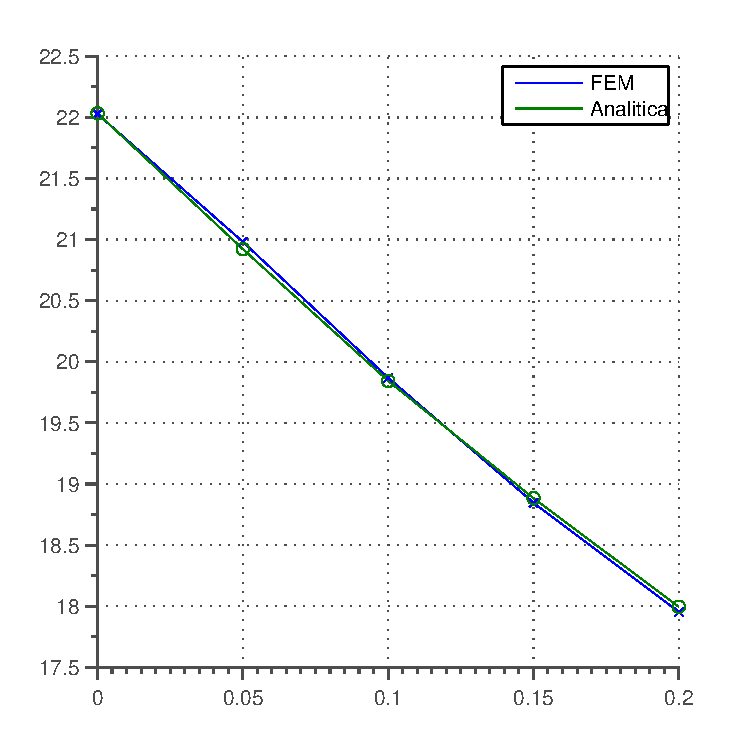
\includegraphics[width=0.7\linewidth]{Simulacoes/Passivo2/validacao_passivo_dx_calibrado.pdf}
	\caption{Validação do modelo, deslocamento axial.}
	\label{fig:validacao_passivo_dx_calibrado}
\end{figure}

Os modelos também foram confrontados com a variação com de parâmetros, no caso, variou-se a largura do ímã e o comprimento do entreferro. A Fig. \ref{fig:validacao_passivo_parametros} compara os resultados em ambos os modelos.

\begin{figure}[th!]
	\centering
	Força de atração (N) x Variação de parâmetros
	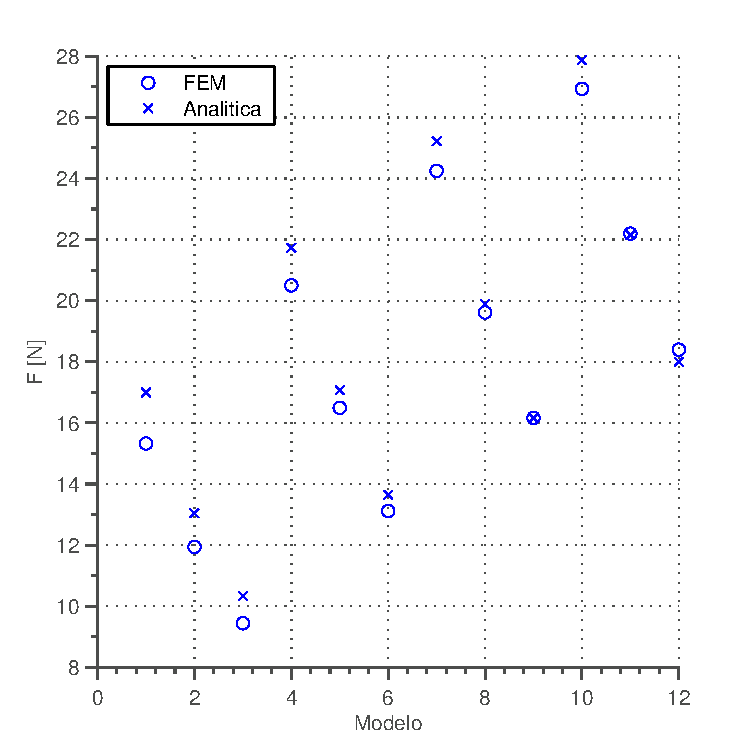
\includegraphics[width=0.7\linewidth]{Simulacoes/Passivo2/validacao_passivo_parametros.pdf}
	\caption{Validação do modelo, variação de parâmetros: largura do ímã e comprimento do entreferro.}
	\label{fig:validacao_passivo_parametros}
\end{figure} 

\section{Otimização dos Parâmetros}

Buscou-se uma combinação de parâmetros que maximizasse a força de atração axial e que minimizasse a força longitudinal. O mancal deve possuir rigidez suficiente para suspender o conjunto inércia, rotor mancal, rotor motor. Estudos realizados estimam um momento de inércia total para o sistema de $6.9 \, 10^{-2} \, kg \, m^2$ com uma massa de 3.52 kg (para operar em ambiente com gravidade). 

O método de otimização utilizado para minimizar o funcional foi o de Nelder-Mead Simplex com restrição de fronteira. Nessa etapa, a otimização foi realizada com o modelo analítico levantado anteriormente, otimizando o tempo de processamento já que a resolução do modelo analítico leva segundos a ser realizado enquanto a do elementos finitos chega a dezenas de minutos.

Os parâmetros escolhidos para a otimização foram todos os que definem construtivamente o circuito passivo do mancal, sendo eles: altura  ($h_{fee}$) e largura  ($w_{fee}$) do ferro estator externo; a altura ($h_m$) e largura ($w_m$) do ímã e largura ($w_{fr}$) do ferro rotor e largura do retorno rotor ($w_{rn}$). Além do comprimento do entreferro ($g_e$) e raio externo do mancal ($r_{eei}$).

Para respeitar a geometria proposta durante a otimização, os parâmetros $w_{fee}$ e $w_{fr}$ não foram manipulados diretamente na otimização, já que não podem assumir valores inferiores a $w_m$ e $w_{rn}$ respectivamente, caso contrário, o mancal encontrado durante a otimização possuiria propriedades distintas da proposta e o modelo analítico seria invalidado. Otimizamos nesse caso, duas componentes $\Delta w_{fee}$ e $\Delta w_{fr}$ que compõem em conjunto com seus pares os comprimentos dos ferros:

\begin{align}
w_{fee}  &= \Delta w_{fee} + w_m \\
w_{fr} &= \Delta w_{fr} + w_{rn}
\end{align}	

Restrições foram impostas para evitar a otimização do mancal para um caso em que a sua construção fosse inviável mecanicamente ou para evitar um mancal que se encontrasse fora das especificações da roda de reação. A Tab. \ref{tab:passivo:restrições} demonstra os valores máximos ($L_{Max}$) e mínimos ($L_{Min}$) impostos para cada elemento do mancal, assim como o valor inicial ($L_0$) utilizado na otimização.


\begin{table}[ht!]
	\centering
	\begin{tabular}{c c c c c c c c c}
		& $h_{fee}$ &$\Delta w_{fee}$ & $w_m$ & $h_m$  & $g_e$ & $\Delta w_{fr}$ & $w_{rn}$ & $r_{eei}$ \\ \hline \hline
		
		$L_{0}$ 	&  6 &   4 &    8 &    10 &   3 &  4 &   6 &    75 \\
		$L_{Min}$ &  2    &  2   &  4  &   5&    1  & 2  &  3&    50\\			
		$L_{Max}$ &  10 &  6 &  12  &   15  &  3  &  8  &   9   &   80		
	\end{tabular} 
	\caption{Valores iniciais, máximos e mínimos utilizado na otimização. Valores em milímetros.}
	\label{tab:passivo:restrições} 
\end{table}

Diversas funções méritos foram testadas visando a obtenção de um mancal que atendesse as especificações. A função pondera seis componentes do mancal, sendo elas: forças de atração em x e y, tamanho do entreferro, raio externo do mancal,  volume ($V_m$) e variação no vetor campo magnético para pequenos deslocamentos ($\Delta B_{g}$).

Buscou-se nessa otimização uma menor força de atração axial ($P_1$) e uma maior força radial ($P_2$). O funcional foi ponderado para privilegiar um maior entreferro ($P_3$) e um menor raio ($P_4$). O volume total ($P_5$) do mancal foi também ponderado no funcional, visando um mancal de dimensões menores. Para obtermos uma força radial linearizada, necessitamos que o vetor campo magnético no entreferro não variasse consideravelmente para pequenos deslocamentos radiais do rotor, o $\Delta B_{g}$ foi ponderado no funcional ($P_6$) . A função mérito (($F$) ) utilizada na otimização está descrito na Eq. \ref{eq:passivo:merito},  os pesos (P) estão separados por importância.

\begin{align}
P_1 &= Fx/2 				\\ 
P_2 &= 125/Fy		\\        
P_3 &= r_{eei}\, 10^3/55 \\     
P_4&= 30/(G_e \,  10^3) \\    
P_5 &= V_m\, 10^6/15 \\        
P_6 &= 25 \,  |{\Delta B_{g}}|\\   
F &= P_1 + P_2 + P_3 + P_4 + P_5 + P_6   \label{eq:passivo:merito}
\end{align}

A Fig. \ref{fig:otimizacao_passivo_parametros} mostra a evolução dos parâmetros ao longo da otimização. Verificamos que a força de atração $F_y$ é maximizada ao longo das interações, porém verificamos que é acompanhada pela força $F_x$ que deveria ser minimizada. Isso ocorre devido a correlação entre as duas forças, sendo que ambas depende do vetor campo magnético acumulado no entreferro ($B_{ge}$). Outra relação direta que é possível ser notada é a do tamanho do entreferro ($g_e$), quanto menor o entreferro menor a relutância do circuito magnético e maior o campo magnético acumulado no entreferro.


\begin{figure}[bh!]
	\centering
	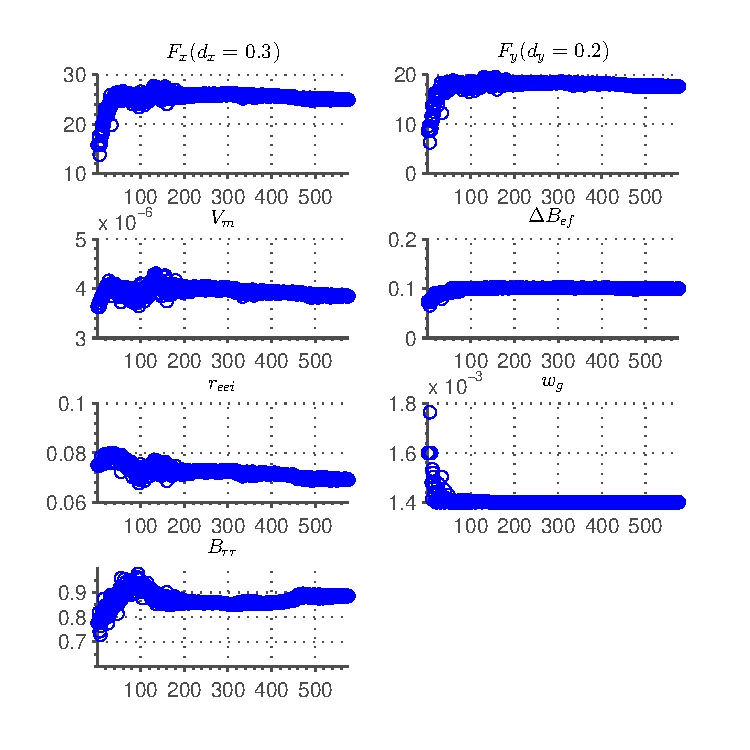
\includegraphics[width=1\linewidth]{Simulacoes/Passivo2/otimizacao_passivo_parametros.pdf}
	\caption{Evolução dos parâmetros ao longo da otimização}
	\label{fig:otimizacao_passivo_parametros}
\end{figure} 

Os pesos da função mérito ao longo da otimização são ilustrados na Fig. \ref{fig:otimizacao_passivo_pesos}, verificamos que os pesos que mais contribuem para o valor do funcional são: P1, P2 que estão relacionados com a força de atração. Em seguida, com uma menor ponderação os demais pesos. 

\begin{figure}[th!]
	\centering
	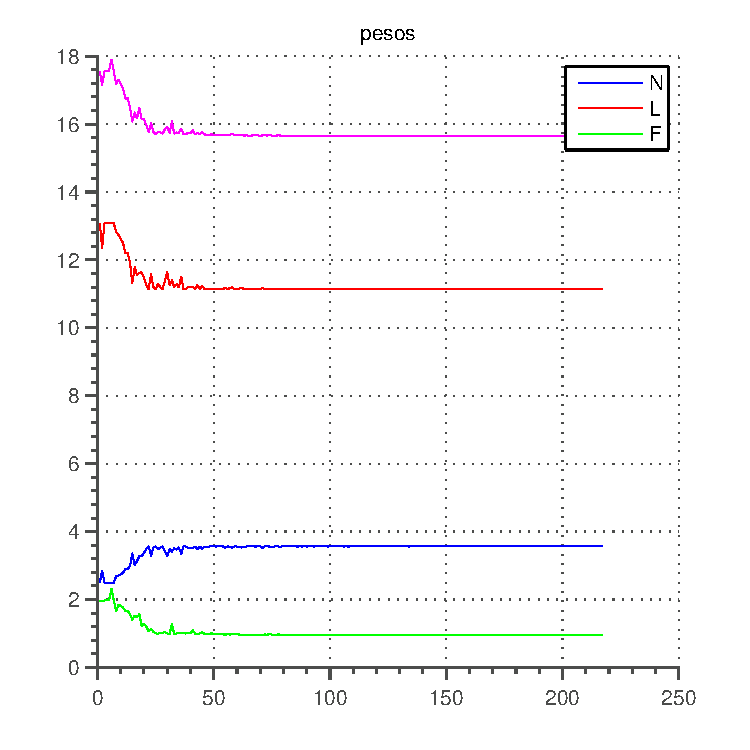
\includegraphics[width=1\linewidth]{Simulacoes/Passivo2/otimizacao_passivo_pesos.pdf}
	\caption{Evolução dos pesos ao longo da otimização}
	\label{fig:otimizacao_passivo_pesos}
\end{figure} 

\section{Mancal Passivo Resultante da Otimização}

As dimensões alcançadas devido a otimização do mancal estão listada na Tab. \ref{tab:passivo:dimensoes:otimizado}, com esses resultados um modelo em elementos finitos foi criado e as forças resultantes levantadas de forma mais precisa (modelo em três dimensões).

\begin{table}[ht!]
	\centering
	\begin{tabular}{c c c c c c c c c}
		& $h_{fee}$ &$\Delta w_{fee}$ & $w_m$ & $h_m$  & $g_e$ & $\Delta w_{fr}$ & $w_{rn}$ & $r_{eei}$ \\ \hline \hline
		$L_{n}$  	&  4.2 &   10 &   10 &    12 &   1.4 &  7 &   6 &    70 \\
	\end{tabular} 
	\caption{Dimensões obtidas devido a otimização. Valores em milímetros.}
	\label{tab:passivo:dimensoes:otimizado} 
\end{table}

Verificamos na Fig. \ref{fig:forca:passivo:otimizado:fem:dx} o resultante  da força devido a translação do rotor em apenas um dos eixos radiais e, também a linearidade da força quando o rotor trabalha em modo diferencial.  

\begin{figure}[!ht]
\centering
\caption*{Força (N) x $\Delta_x$ (mm) - Deslocamento Radial: y = 0, z = 0}
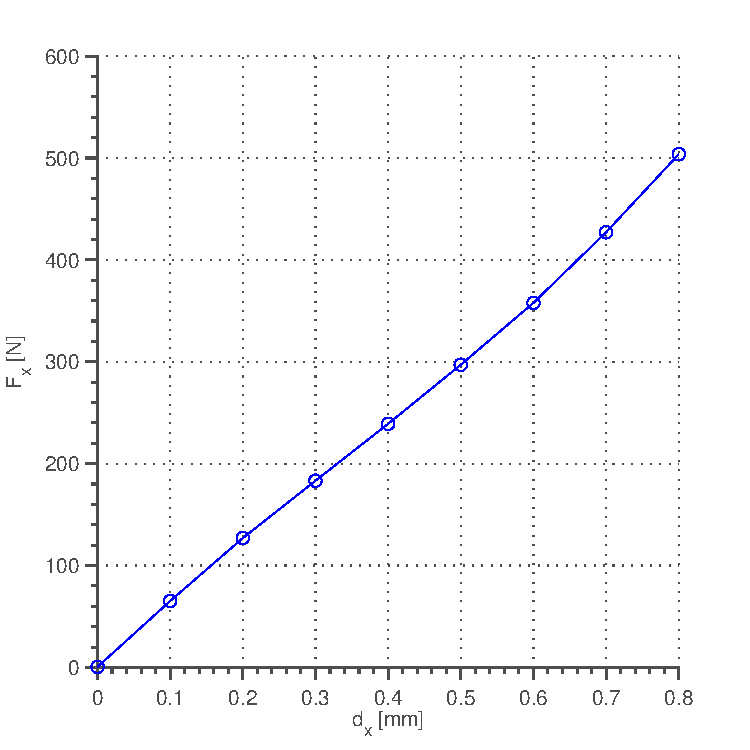
\includegraphics[width=0.6 \columnwidth,angle=0]{Figs/Simulacoes/Passivo2/fem/passivo_otimizado_fem_dx}
\caption{Força atuante no rotor dado uma translação radial}
\label{fig:forca:passivo:otimizado:fem:dx}
\end{figure} 

A força gerado pela translação axial é ilustrada na Fig. \ref{fig:forca:passivo:otimizado:fem:dy}, essa força restaurativa torna a parte passiva do mancal estável e é a responsável pela rigidez nesse grau de liberdade. Notamos que a força necessária para deslocar 1 mm axialmente quando o mancal está no ponto de operação é de aproximadamente 140N. Verificamos que a força possui um componente diferente de zero quando o rotor está alinhado com o estator externo (z = 0), diferente do encontrado via  modelo analítico, explica-se esse fenômeno pelo erro numérico causado pela malha de cálculo.

\begin{figure}[!ht]
	\centering
	\caption*{Força (N) x $\Delta_z$ (mm) - Deslocamento axial: x = 0, y = 0}
	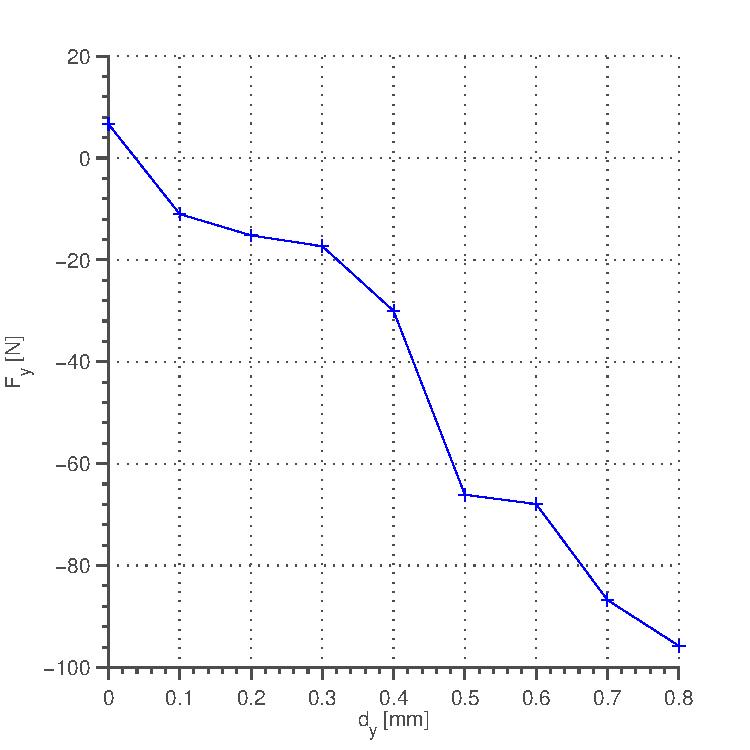
\includegraphics[width=0.6 \columnwidth,angle=0]{Figs/Simulacoes/Passivo2/fem/passivo_otimizado_fem_dy}
	\caption{Força atuante no rotor dado uma translação axial}
	\label{fig:forca:passivo:otimizado:fem:dy}
\end{figure}

Um mapa do módulo da força radial no plano x,y é ilustrado na Fig. \ref{fig:passivo_otimizado_fem_plano}, notamos que em torno do ponto de operação a força é praticamente nula. Porém, quando o rotor encontra-se em algum de seus extremos, a força de atração é da ordem de centenas de Newton o que influencia na definição do circuito ativo que tem que ser capaz de vencer essa força.

\begin{figure}[!ht]
\centering
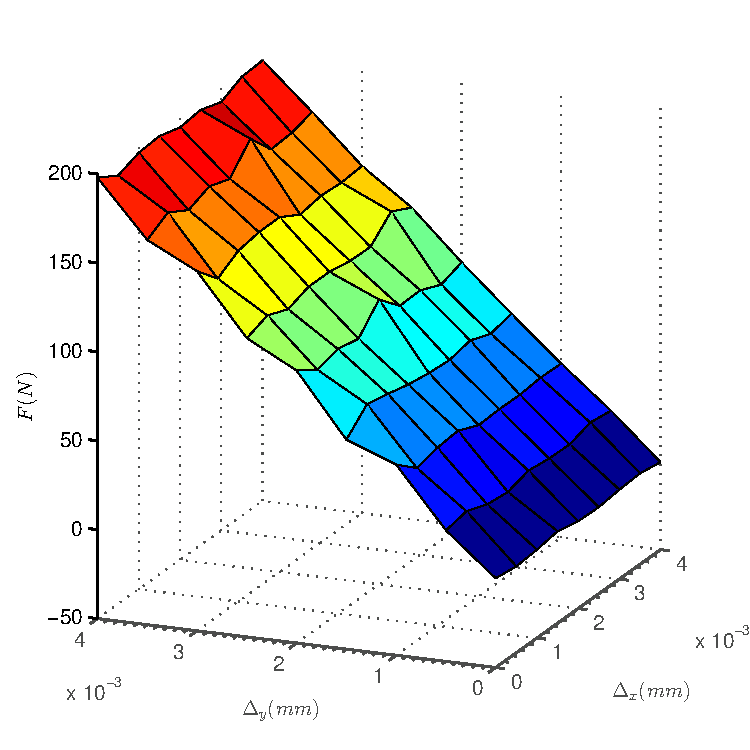
\includegraphics[width=0.7\linewidth]{Figs/Simulacoes/Passivo2/passivo_otimizado_fem_plano}
\caption{Mapa de forças devido ao descolamento radial}
\label{fig:passivo_otimizado_fem_plano}
\end{figure}


A Fig. \ref{Fig:Modelagem:Curva:passivo:dy:linhas} ilustra o resultado da simulação através de elementos finitos onde o rotor é transladado verticalmente a 0.8 mm. Verificamos que as linhas de campo não sofrem inclinação proporcional ao deslocamento do rotor, essas deformações apresentam um erro no modelo analítico já que supusemos na Subsec. \ref{SubSec:CampoX/Y} que as linhas de campo poderiam ser decompostas em x e z e que essa decomposição é diretamente relacionada com o deslocamento do rotor ($\theta$). 

\begin{figure}[!ht]
	\centering
	\subfloat[t][$\Delta_x = 0 mm$ e $\Delta_z = 0mm$]
	{
		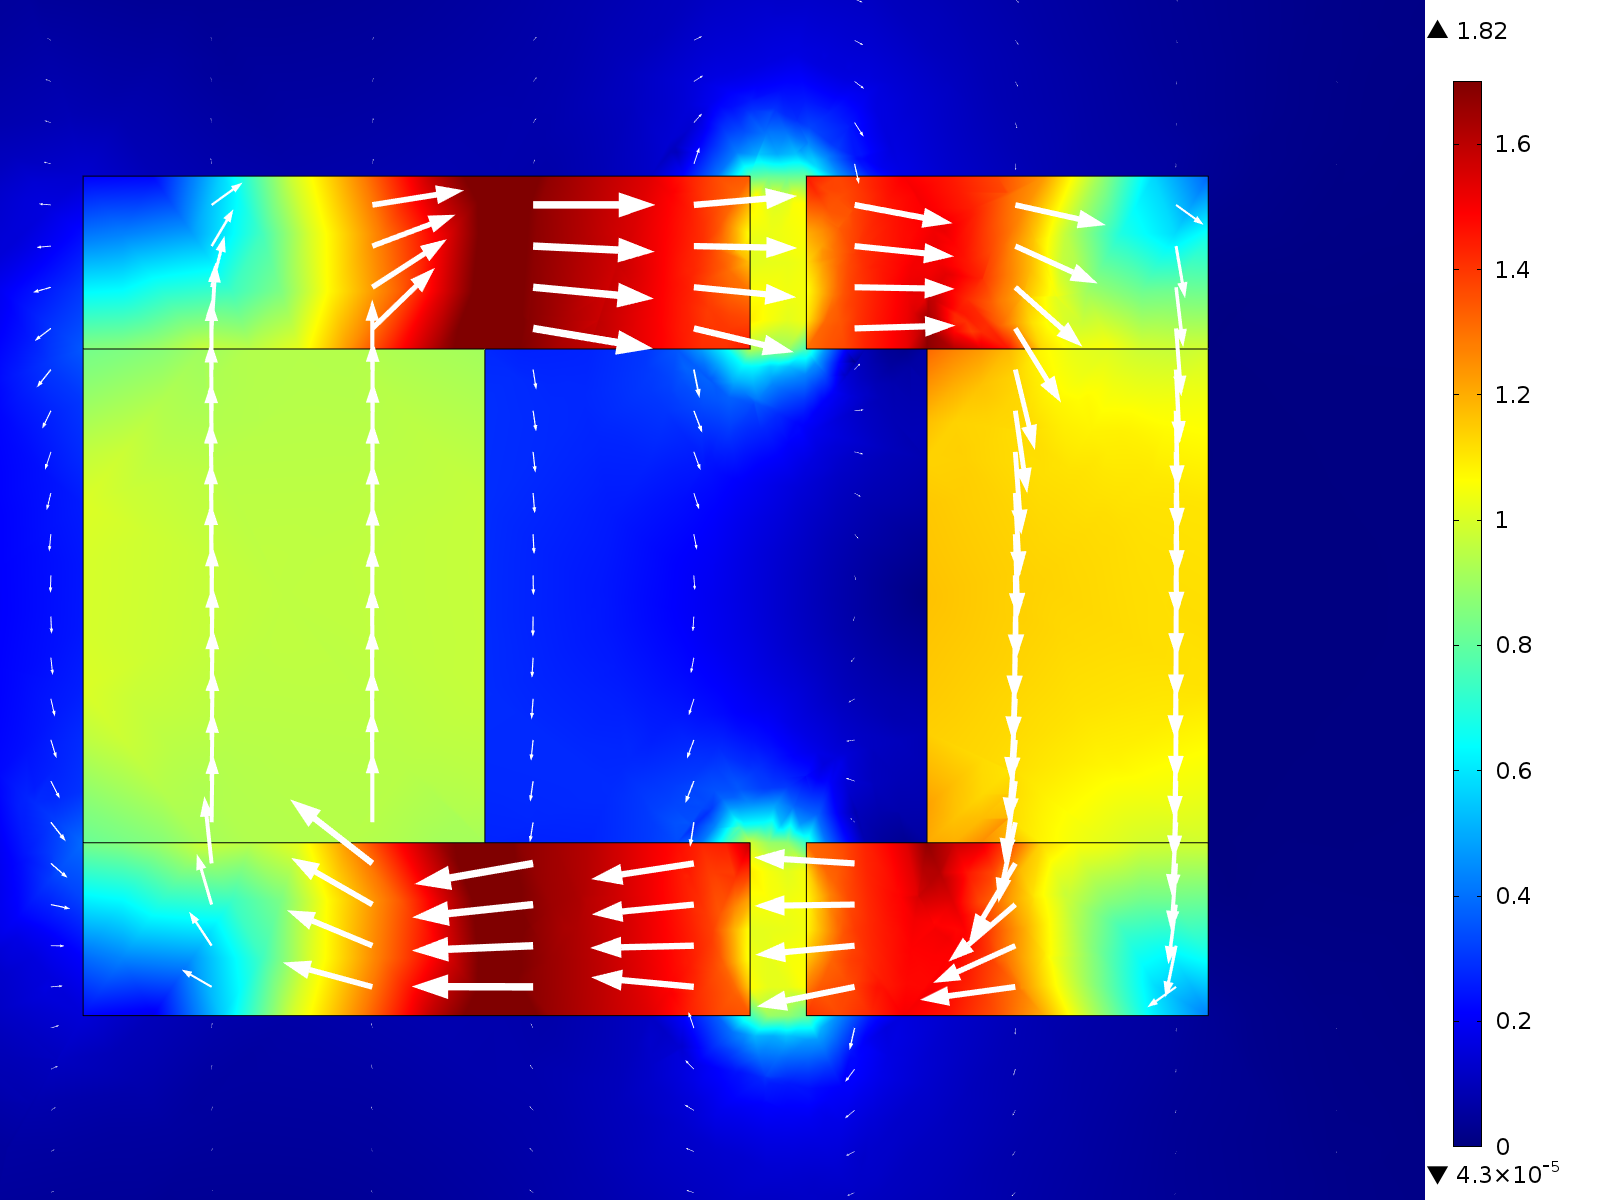
\includegraphics[width=0.5\linewidth]{Figs/Simulacoes/Passivo2/fem/dy_00}
	}	\label{Fig:Modelagem:Curva:passivo:dy:linhas:0}
	\subfloat[t][$\Delta_x = 0 mm$ e $\Delta_z = 0.8$]
	{
		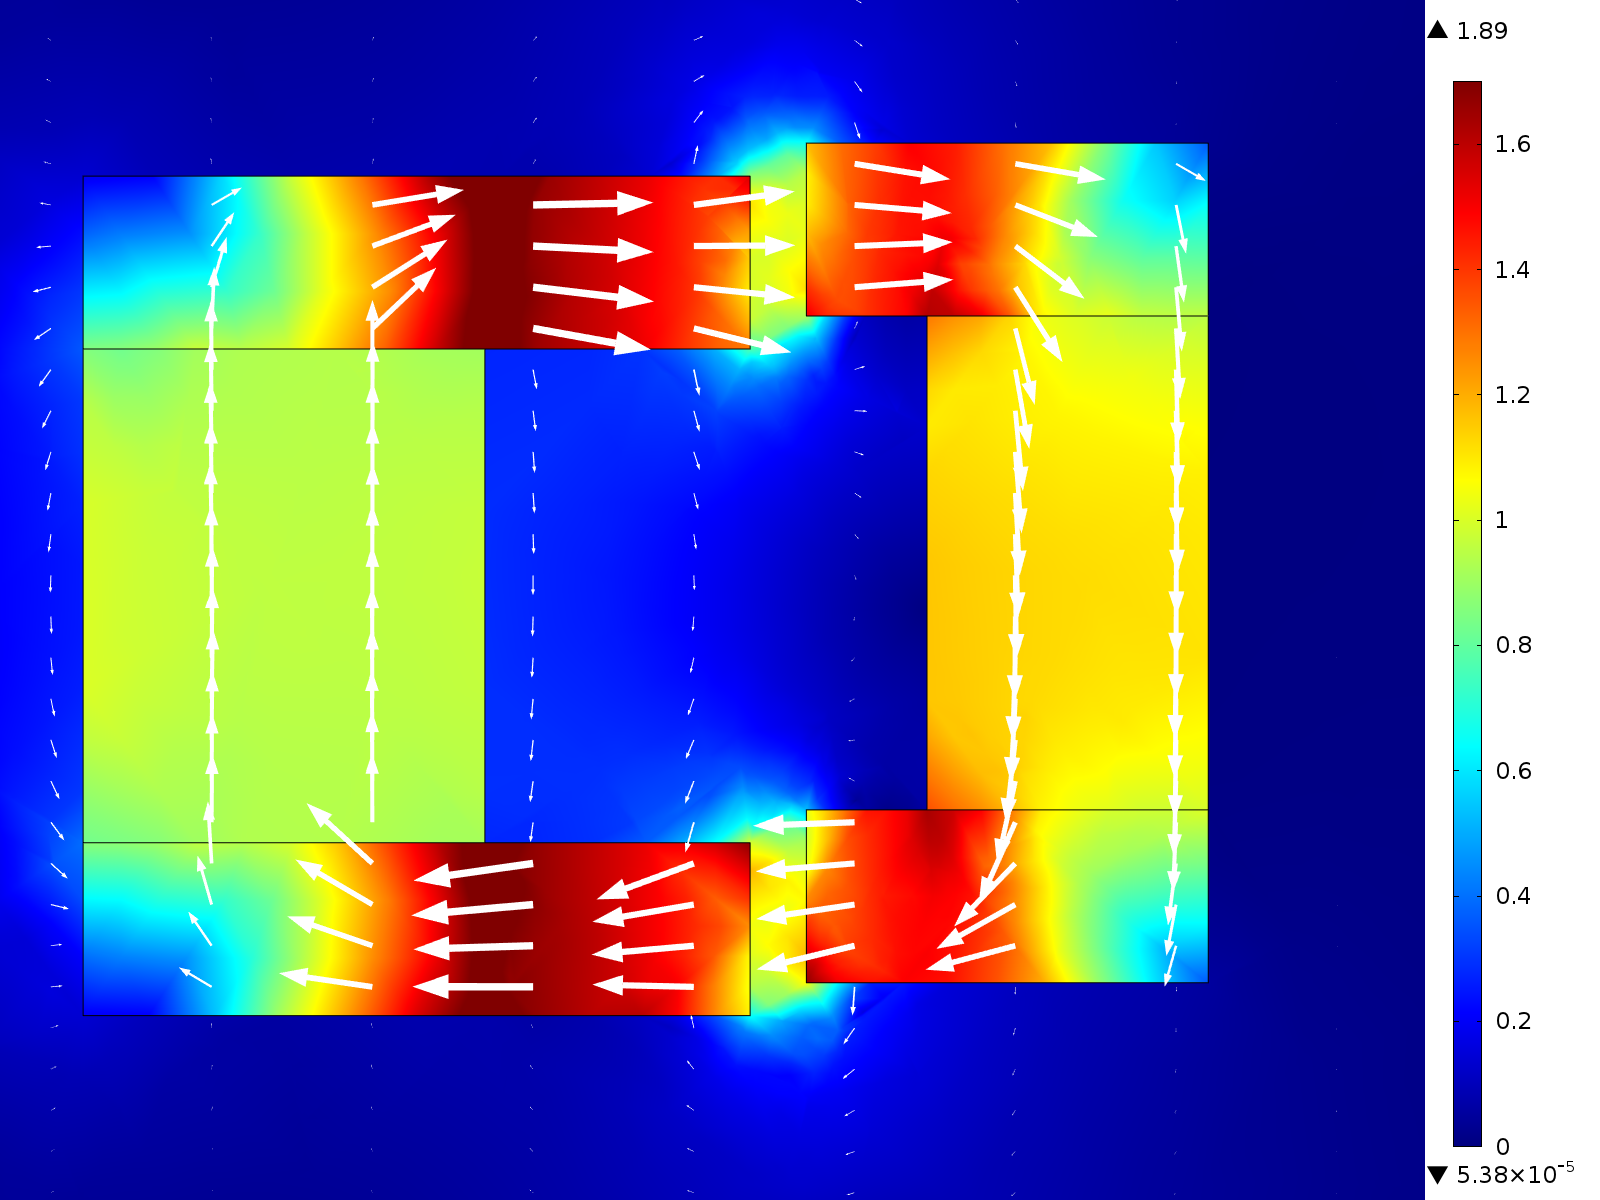
\includegraphics[width=0.5\linewidth]{Figs/Simulacoes/Passivo2/fem/dy_08}
	}	\label{Fig:Modelagem:Curva:passivo:dy:linhas:1,2}
	\caption{Campo magnético via simulação em elementos finitos para deslocamentos na vertical}
	\label{Fig:Modelagem:Curva:passivo:dy:linhas}
\end{figure}

Na Fig. \ref{Fig:Modelagem:Curva:passivo:dx:linhas} o resultado da simulação FEM para o deslocamento radial do rotor. Notamos nessa simulação que o fluxo magnético é contido nos ferros e que ocorre pouca dispersão das linhas de campo. Observamos, também a saturação dos ferros em todos os casos, essa saturação é necessária para forçar a linearidade da força de atração quando trabalhado em modo diferencial. Além disso,  verificamos que a área do entreferro ($S_g$) possui um pequeno espraiamento causando um aumentado no volume em que o campo magnético está acumulado e por consequência um aumento na força. 
%\todo{confusa a relação da última frase com o começo do paragrafo}


A massa do rotor (m) é calculada pelo volume obtido das otimizações, sendo o volume 47940 $mm^6$ e a densidade do material utilizado como $7.8$ [g/$mm^3$], a massa do sistema é:

\begin{align}
	m = 0.375 \; [Kg]
	\label{eq:massa}
\end{align}


\subsection{Estabilidade em Tilt}

Verificada a estabilidade na inclinação axial, pudemos projetar em dois movimentos distintos: deslocamento radial e axial. Dado a propriedade plana do mancal proposto, obtivemos um grande deslocamento axial comparado com o radial, gerando assim a estabilidade do rotor. Para o caso da inclinação máxima do rotor (um grau, limitada pelo batente) o deslocamento radial é de $0.0107$ mm e o deslocamento axial de $1.2$ mm axial, gerando assim uma recuperação rápida axial, o que impede o rotor de entrar em instabilidade.

Em simulação de elementos finitos, calculamos que o torque restaurativo para uma inclinação de um grau em torno de um dos eixos é de $3 N.m$, ou seja, o resultante da força em z devido a inclinação é de 42N. O gráfico da Fig. \ref{fig:passivo:torque:tilt} demonstra a força restaurativa gerada devido a aplicação de uma série de inclinações.

\begin{figure}[!ht]
\centering
\caption*{Torque (N.m) por inclinação (grau) }
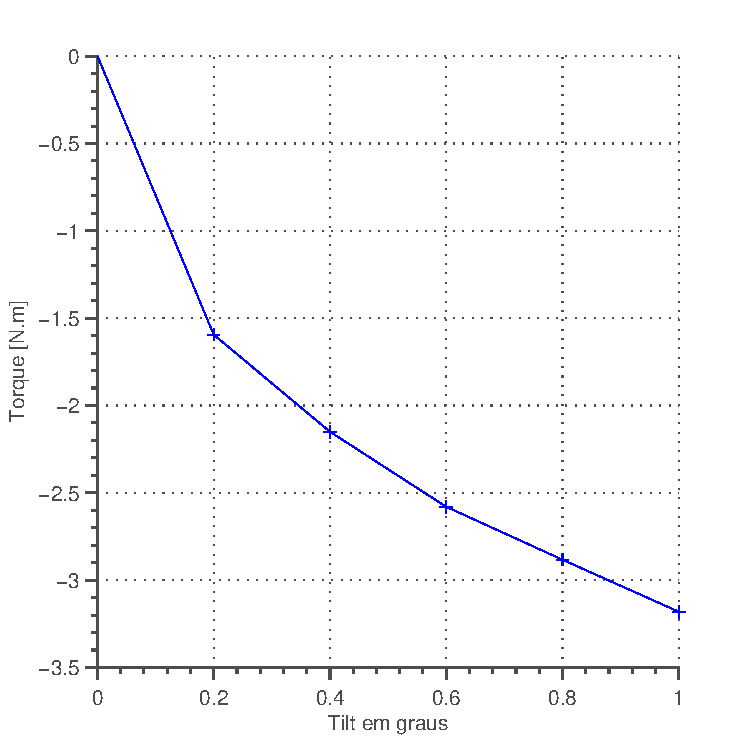
\includegraphics[width=0.7\linewidth]{Figs/Simulacoes/Passivo2/fem/passivo_otimizado_fem_tilt}
\caption{Torque resultante da inclinação do rotor}
\label{fig:passivo:torque:tilt} 
\end{figure}


